\documentclass[10pt,a4paper]{article}
\usepackage[a4paper, left=3cm, right=3cm, top=3cm, bottom=3cm, headsep=10mm, footskip=12mm]{geometry}
\usepackage[T1]{fontenc}
\usepackage[ngerman, english]{babel}    % mehrsprachiger Textsatz
% babel: letzte Sprache in Optionen zeigt die Sprache des Dokumentes
% und kann durch den Befehl \selectlanguage{} geaendert werden
% Passen Sie die Optionen des babel-Paketes nach Bedarf an!
\usepackage{float}
\usepackage{graphicx}
\usepackage{url}
\usepackage{pdflscape}
\usepackage{mathtools}
\usepackage{amssymb, amsmath, amstext}
\usepackage{amsthm}
\usepackage{xcolor}
\usepackage{nameref}
\usepackage{siunitx}
\usepackage{makecell}
\usepackage{hyperref}
\usepackage{enumitem}
\usepackage[superscript,biblabel]{cite}
\usepackage{caption}
\usepackage{subcaption}
\usepackage{tabularx} 			% Tabellen erzeugen
\usepackage{multirow}			 % Zeilen in Tabellenbearbeitung
\usepackage{multicol} 			% Spalten in Tabellenbearbeitung 
\usepackage{lmodern}                        % Ersatz fuer Computer Modern-Schriften 
\usepackage{amsmath}                                           % zum besseren Aussehen am Bildschirm
\usepackage{booktabs} % für schönere Tabellen
\usepackage{sidecap}
\usepackage{rotating} % für die Landscape-Umgebung
\usepackage{afterpage}
\definecolor{Bluetitle}{HTML}{1F3864}
\definecolor{softbluetitle}{HTML}{274D7E}
\definecolor{Greyish}{HTML}{5A5A5A}
\renewcommand{\refname}{Reference}
\usepackage{array,multirow}
\newcommand{\specialcell}[2][c]{%
	\begin{tabular}[#1]{@{}c@{}}#2\end{tabular}}




\begin{document}
	
	\begin{titlepage}
		\begin{center}
			\begin{figure}[h!tbp]
				
\includegraphics[width=\linewidth]{HUlogo.PNG}
			\end{figure}
			\vspace*{2 cm}
			
			\textcolor{Bluetitle}{\textbf{\huge Atmung und Gärung}}\par
			
			\vspace*{2cm}
			
			\textcolor{Greyish}{\textbf{Versuchsdurchführende}}\par
			\textcolor{Greyish}{Oscar Moore (634083)}\par
			\textcolor{Greyish}{Fridolin Rehnig (625757)}\par
			\textcolor{Greyish}{Philipp Kunze (625468)}\par
			\textcolor{Greyish}{Daniel Kollenkirchen (625426)}\par
			\textcolor{Greyish}{Huyen Anh Nguyen (572309)}\par
			
			\vspace*{0.5cm}
			\textcolor{Greyish}{\textbf{Versuchsort}}\par
			\textcolor{Greyish}{Campus Nord, Haus 9}\par
			\textcolor{Greyish}{R2001}\par
			\vspace*{0.5cm}
			\textcolor{Greyish}{\textbf{Versuchsbetreuer}}\par
			\textcolor{Greyish}{Dr. Boris Hedtke}\par
			
			\vspace*{2 cm}
			
			\textcolor{Greyish}{02. Juli 2024}\par
			
			
			
			
		\end{center}
	\end{titlepage}
	
	\tableofcontents
	
	\section{Einführung}	
		In diesem Versuchskomplex werden der Glucose- und Sauerstoffverbrauch von Hefekulturen unter verschiedenen Bedingungen untersucht, um die Unterschiede zwischen Atmung und Gärung zu verstehen. Hefen eignen sich hierfür perfekt, da sie fakultativ anaerob und daher in der Lage sind, Energie sowohl durch Atmung in Gegenwart von Sauerstoff als auch durch Gärung unter anaeroben Bedingungen zu gewinnen.  Ziel ist es, die Effekte von Sauerstoffverfügbarkeit und Inhibitoren auf den Energiestoffwechsel der Hefe zu analysieren und dadurch die Energiegewinnung in Hefezellen unter unterschiedlichen Umweltbedingungen besser zu verstehen.\\
		Der Versuch wird in zwei Hauptteile geteilt:\\
		Im ersten Teil wird, anhand von der Glucosekonzentration, der Glucoseverbrauch von Hefesuspensionen unter aeroben und anaeroben Bedingungen gemessen. Das Ziel ist ein Vergleich, bzw. Unterscheidung der Suspensionen anhand des Glucoseverbrauchs.
		Zudem wird gravimetrisch die Gewichtsabnahme einer rein anaeroben Hefesuspension gemessen. Die Zielsetzung des Versuchs ist die Prüfung, ob man mit der Gewichtsabnahme eine CO2-Abnahme effektiv bestimmen kann. \\
		Hier ist ein theoretisches Verständnis des Pasteur- und des Crabtree-Effekts besonders wichtig. Der Pasteureffekt besagt, dass unter zunehmend anaeroben Bedingungen der Glucoseverbrauch ansteigt, bis zur 15- bis 16-fache Menge. Dies soll bedingt sein dadurch, dass in aeroben Bedinungen in den Mitochondrien Pyruvat vollständig oxidativ abgebaut wird, jedoch in anaerober Umgebung nicht vollständig oxidiert wird und, ohne ATP-Bildung, in Endprodukte wie Milchsäure, Ethanol, Propionsäure umgesetzt wird. Der Crabtree-Effekt beschreibt, dass selbst in hoher Sauerstoffverfügbarkeit, gleichzeitig mit der Atmung eine Alkoholgärung auftritt. Vermutlich wird den Hefen, durch den schnellen Abbau von Glucose zu Ethanol ein Vorteil gegenüber Konkurrenten. Dieses gleichzeitige Ablaufen von Gärung und Atmung führt zu einem starken Anstieg des respiratorischen Quotienten. \\
		\\
		Im zweiten Teil wird der Sauerstoffverbrauch von Hefe- und Tabakpflanzen-Gewebesuspension, mithilfe einer Clarkelektrode unter anaerobe Bedingung gemessen. Zudem wird beide Gewebesuspensionen miteinander verglichen, welche mit Kaliumcyanid versetzt wurde. \\
		Das Ziel ist zu ermitteln, wie sich der Sauerstoff von Hefe und Pflanzen unterscheidet und wie sich Kaliumcyanid, einem Cytochromoxidase-Hemmstoff, auf den Sauerstoffverbrauch der Suspensionen auswirkt.\\
		 In Flüssigkulturen, die nicht ständig Sauerstoff ausgesetzt sind, wie in diesem Versuch, kommt es zum schnellen Verbrauch des Sauerstoffs, da die Sauerstoffkonzentration begrenzt ist durch die Löslichkeit des Sauerstoffs in Wasser welches ca. 8mg pro Liter beträgt. In der Atmungskette ist die terminale Oxidase die Cytochromoxidase, welche eine hohe Sauerstoffaffinität hat. Bei der Zugabe von Cyanid-Ionen wird das Enzym Cytochromoxidase gehemmt. Bei höheren Pflanzen gibt es eine cyanidresistente Atmung über die Alternative Oxidase, welche direkt aus dem Ubiquinonpool Elektronen bezieht. Die ATP-Regenerierung ist jedoch geringer und durch die teilweise Entkopplung des Protonen- und Elektronentransports wird die Energiedifferenz in Form von Wärme frei.\\
		 

	
	\section{Material und Methode}
	Es wurde wie im Skript beschrieben verfahren, lediglich für den zweiten Versuchsteil wurden beim Erstellen der Hefelösung, 0,52g Hefe und 2,01g Glukose abgewogen. Beim ansetzen der Pflanzenzellsuspension, wurden 1,51g Glukose und 5,25g der BY2-Pflanzenzellkulturen verwendet.
	
	\section{Ergebnis}
	\subsection{Aerobe und anaerobe Glucoseverbrauch}
	Es wurde 1.8g Glucose in 250mL Medium gelöst, welches eine Anfangskonzentration von 40mM ergibt.\\
	
		\begin{table}[H]
		\centering
		\caption{Glucosekonzentration im Medium von Backhefe in aerobe und Anaerobe Bedingungen. Die Konzentration wurde vom Skala in Figure \ref{fig: Glucoseverbrauch} abgelesen.}
		\label{tab:glucoseconc anareob und aerob}
		\begin{tabular}{ccc}
			\toprule
			\multirow{2}{*}{t in min} & \specialcell[t]{c(Glucose) bei \\ aerobe Bedingung in mM}& \specialcell[t]{c(Glucose) bei \\anaerobe Bedingung in mM}\\
			\midrule
			10 & 111 & 55\\
			15 & 55 & 28\\
			20 & 14 & <14\\
			25 & 5.5 & 0\\
			\bottomrule
		\end{tabular}
	\end{table}	
	Der Glucoseverbrauch in Table \ref{tab:Glucoseverbrauch} wurde nach Gleichung (\ref{eq: Glucoseverbrauch}) bestimmt. \\
	Die letzte Konzentration wurde bei t = 25 Minuten bestimmt.
	\begin{equation}\label{eq: Glucoseverbrauch}
		\Delta c(Glucose) = c_0(Glucose) - c_{end}(Glucose)
	\end{equation}
	
	\begin{table}[H]
		\centering
		\caption{Glucoseverbrauch von Backhefe bei aerobe und anaerobe Bedingungen nach 25 Minuten.}
		\label{tab:Glucoseverbrauch}
		\begin{tabular}{ccc}
			\toprule
			& $\Delta$c(Glucose) & Glucoseverbrauch pro 1g Hefe\\
			\midrule
			aerobe Bedingung & 1.38 mM/ min & 6.39 mmol/ min g Hefe\\
			anaerobe Bedingung & 1.60 mM/min & 7.41 mmol/min g Hefe\\
			\bottomrule
		\end{tabular}
	\end{table}	
	
	\subsection{Anaerobe Gährung}
	Die wiederholte Messung des Gewichts im Abstand von 10 min sowie die daraus resultierende Abnahme der Stoffmenge von Glukose (siehe Gleichung \ref{eq:anareobeglucoseverbrauch}) wurde in Table \ref{tab:anaerobe glucoseverbrauch} dargestellt. Die Abnahme der Stoffmenge der Glukose je Gramm Hefe konnte einfach abgeleitet worden, da genau 1 Gramm Hefe genutzt wurde. Aus diesem Wert konnte ein Diagramm im zeitlichen Verlauf erstellt werden (siehe Figure \ref{fig:wurzel ohne P}). Es zeigte sich, dass die ersten zwei Messpunkte (nach 0 und 12 min) nicht in den Verlauf des Verbrauchs passte. Aber auch der Messwert nach 52 min weicht von dem restlichen Verlauf ab. Es wurde mittels einer linearen Regression durch die Messpunkte ab Messpunkt 3 (22 min) der durchschnittliche Glukoseverbrauch ermittelt. Dabei entspricht der Anstieg der linearen Regressionsgeraden dem Verbrauch. Dementsprechend konnte ein Glukoseverbrauch von 0,1686 mmol Glukose pro Minute und Gramm Hefe festgestellt werden. Der Bestimmtheitsgrad der linearen Regression liegt bei R² = 0,97.
	
	\begin{table}[H]
		\centering
		\caption{Glucoseverbrauch von Backhefe bei aerobe und anaerobe Bedingungen nach 25 Minuten.}
		\label{tab:anaerobe glucoseverbrauch}
		\begin{tabular}{cccccc}
			\toprule
			\multirow{2}{*}{Uhrzeit [hh:mm]}& t in min & m in g & $\Delta$ Gewicht & $\Delta$ n(Glucose) & $\Delta$n(Glucose)/g Hefe\\
			& && in mg & in mmol&  in mmol/g\\
			\midrule
			15:49 & 0 & 72.1833 & 0 & 0 & 0\\
			16:01 & 12 & 72.1817 & 16 & 0.1818 & 0.1818\\
			16:11 & 22 & 72.1779 & 54 & 0.6136 & 0.6136\\
			16:21 & 32 & 72.1689 & 144 & 1.6363 & 1.6363\\
			16:31 & 41 & 72.1602 & 231 & 2.6250 & 2.6250\\
			16:42 & 52 &72.1356 & 477 & 5.4205 & 5.4205\\
			16:52 & 62 & 72.1207 & 626 & 7.1136 & 7.1136\\
			\bottomrule
		\end{tabular}
	\end{table}	
	
	\begin{equation}\label{eq:anareobeglucoseverbrauch}
		\text{Abnahme der Stoffmenge von Glucose} [mmol]= \frac{1 mmol   \text{ Glucose}}{88mg  \text{ CO}_2} \cdot \text{Abnahme des Gewichts}[mg]
	\end{equation}
	
	\begin{figure}[H]
		\centering
		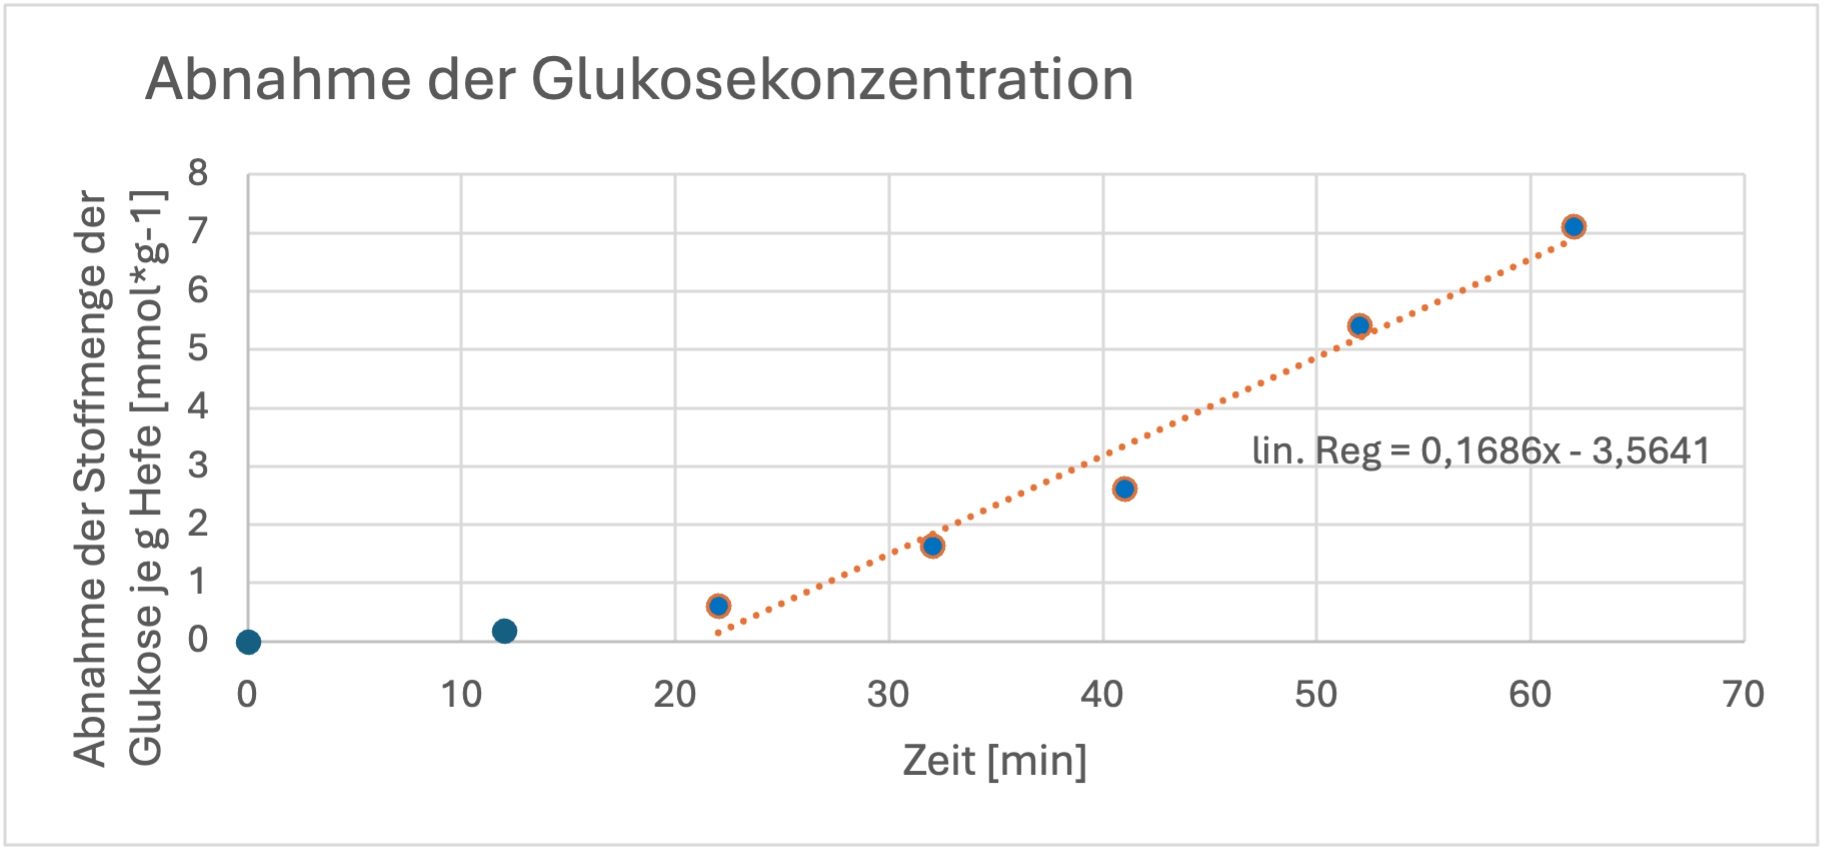
\includegraphics[scale=1]{anaerobe_GluConc.png}
		\caption{Abnahme der Stoffmenge der Glukose je g Hefe abhängig von der Zeit mit linearer Regression durch die Werte ab 22 min..}
		\label{fig:wurzel ohne P}
	\end{figure}
	
	\subsection{Sauerstoffverbrauch und cyanidresistente Atmung}
	Der Verbrauch von Sauerstoff wird aus der Steigung im linearen Bereich in Figure \ref{fig: Sauerstoffverbrauch} bestimmt. 
		\begin{table}[H]
		\centering
		\caption{Sauerstoff- und Glucoseverbrauch von Backhefe und BY2-Pflanzenzellen in anaeroben Bedingungen mit und ohne Zugabe von Kaliumcyanid.}
		\label{tab:O2verbrauch und CN}
		\begin{tabular}{ccc}
			\toprule
			& $O_2$-Verbrauch in $\mu$g/min g Cells& Glucose-Verbrauch in mmol/ min g Cells\\
			\midrule
			Hefe ohne KCN & 311.4 & 3.244 $\cdot$ 10$^{-3}$\\
			Hefe mit KCN & 54.42& 5.669 $\cdot$ 10$^{-4}$\\
			& & \\
			BY2 ohne KCN & 2.753 & 2.868 $\cdot$ 10$^{-5}$\\
			BY2 mit KCN & 3.796& 3.954 $\cdot$ 10$^{-5}$\\
			\bottomrule
		\end{tabular}
	\end{table}	
	
	\section{Diskussion}
	\subsection{Backhefe bei aerobe und anerobe Bedingungen}
		Wie in Table \ref{tab:Glucoseverbrauch} zu sehen, verbraucht Hefe unter anaeroben Bedingungen mehr Glukose als die unter aeroben Bedingungen. Diesen Effekt wird auch als Pasteur-Effekt bezeichnet, wo unter anaeroben Bedingungen Hefen und andere Mikroorganismen verstärkt Zucker abbauen, um den Energiegehalt innerhalb der Zelle aufrecht zu erhalten. \\
		Der Crabtree-Effekt beschreibt das Betreiben von Gärung, selbst wenn Sauerstoff vorhanden ist. Das Betreiben von beiden Prozessen, sowohl Gärung als auch Atmung hilft der Hefe noch schneller Energie produzieren zu können und gleichzeitig andere Mikroorganismen wie konkurrierende Bakterien durch die Gärungsendprodukte wie Ethanol abtöten zu können. Dies erklärt möglicherweise den geringen Unterschied des Glukose Verbrauchs zwischen der aerob und anaerob gehaltenen Hefe während des Versuchs 1A. Bestätigen kann dieser Effekt aber nicht. Um den Crabtree-Effekt nachzuweisen, müsste der Ethanolgehalt im Medium gemessen werden.\\
		Für uns Menschen ist der Prozess der aeroben Gärung (Crabtree-Effekt) ein wirtschaftlicher Faktor, der zum Genuss von alkoholischen Getränken wie Bier und Wein führt.\\
		Die aerobe Atmung produziert circa 30-36 ATP-Moleküle/Glucose durch die Glycolysis, Citratzyklus und Atmungskette, während die anaerbe Atmung (Gärung) nur 2 ATP-Moleküle/Glucose produziert.\\
		
		\begin{equation}\nonumber
			Atmung \quad C_6H_{12}O_6 + 6 O_2 \rightarrow 6 CO_2 + 6 H_2O
		\end{equation}
		\begin{equation}\nonumber
			Gärung \quad C_6H_{12}O_6 + 2 ADP + 2P_i \rightarrow 2 C_2H_5OH + 2 CO_2 + 2 ATP
		\end{equation}
	\\
		Der Glucoseverbrauch die gemessen wurden, können von den realen Werten abweichen, da bei der Durchführung das Gefäß für die anaorobe Bedingung nicht komplett verschlossen war. Zudem wurden die Werte der Glucoseteststreifen zu Beginn nicht sofort abgelesen, weswegen die Farben über die Zeit dunkler wurden.
		
		
	\subsubsection{anaeorbe Gärung}	
	Bei der Gärung unter anaeroben Bedingungen wird laut dem Pasteur-Effekt mehr Glukose verbraucht als während der Zellatmung unter aeroben Bedingungen. Laut dem Crabtree-Effekt nutzt Saccharomyces cerevisiae unter aeroben Bedingungen sowohl die Zellatmung als auch die Gärung, um möglichst viel Energie zu gewinnen. Dennoch ist zu erwarten, dass bei der Gärung unter anaeroben Bedingungen mehr Glukose verbraucht, wird als unter aeroben Bedingungen. Wenn 1 mmol Glukose vergoren werden würde, so würde man eine Gewichtsabnahme von 88 mg erwarten können. Das lässt sich durch umstellen der Gleichung  \ref{eq:anareobeglucoseverbrauch} nach dem Gewichtsverlust ermitteln (siehe Gleichung  \ref{eq:Verbrauch}). Die gravimetrische Messung zeigt im, Vergleich zu den ersten Teil des Versuches, einen deutlich geringeren Verbrauch von Glukose. Während der Glukoseverbrauch bei Versuch "Aerobe und anaerobe Glucoseverbrauch" bei 1,6 mmol/l/min lag, so lag er bei der gravimetrischen Bestimmung bei nur 0,1686 mmol/g/min. Wie im vorherigen Teil bereits erläutert, kann es durch den Versuchsaufbau im Teil A zu Ungenauigkeiten kommen. Ergänzend dazu, ist die Farbe der Teststreifen nicht ganz genau bestimmbar und auch die vom Hersteller bereitgestellte Farbskala enthält nicht alle Farbnuancen.\\ Dementsprechend ist die Ermittlung der Glukose-Konzentration durch die Teststreifen eine eher ungenaue Messmethode und dient nur zur Schätzung. Eine gravimetrische Bestimmung mithilfe einer Feinwaage, welche bis auf ein tausendstel Gramm messen kann, ist im Vergleich dazu eine deutlich genauere Messmethode. Jedoch kann es auch hier zu Fehlern kommen. Zum einen befand sich in dem für den Versuch verwendeten Kunststoffschlauch Wasserrückstände, die durch die Veränderung des Gasvolumen bewegt wurden. Durch diese Gewichtsverlagerung kann die Messung verfälscht sein. Zum anderen ist der Zustand der Waage anzumerken. Die Waage zeigte in regelmäßigen Abständen Fehlermeldungen, wodurch begründete Zweifel an der Funktionstüchtigkeit dieser Waage nicht ausgeschlossen werden können. Da die berechneten Werte des Glukoseverbrauchs in Versuch 1A und Versuch 1B eine Abweichung um den Faktor 10 zeigten, lassen sich die Werte nur schwer miteinander vergleichen. Bei der Verlässlichkeit der Testmethoden würde, mit Blick auf die evtl. defekte Waage, eher die Nutzung der Glukose-Teststreifen sinnvoll erscheinen. Wenn es um die Genauigkeit der Messung geht, würde jedoch ganz klar die gravimetrische Bestimmung das Mittel der Wahl sein.
	
	\begin{equation}\label{eq:Verbrauch}
			\text{Abnahme des Gewichts}  [mg] = \frac{\text{Verbrauch von } 1 mmol Glucose}{1 mmol \text{Glucose}} \cdot 88mg
	\end{equation}

		
	\subsection{Sauerstoffverbrauch und cyanidresistende Atmung}
	Der Glucoseverbrauch im Medium ist bei der Backhefe deutlich höher als bei der Pflanzenzelle BY2. Anders als die Hefe besitzen Pflanzenzellen ein hohen Glucosespeicher in den Vakuole, welches für die Atmungskette verwendet werden kann. Der niedrige Sauerstoffverbrauch bei den  Pflanzen liegt an der Diffusionsrate von Sauerstoff in der Flüssigkeit durch die Zellwand. \\
	Die Hefezellen verbrauchen innerhalb von 13 Minuten das ganze Sauerstoff in der Lösung. Der Glucoseverbrauch ist hier aber nicht Vergleichbar mit der Gärung in Aufgabe 1, da hier nur der Sauerstoffverbrauch bestimmt wurde und aus dem Sauerstoffverbrauch der Glucoseverbrauch bestimmt wurde. Somit kann der Glucoseverbrauch nur auf einem aeroben Stoffwechsel zurück geführt werden.\\
	Die Zugabe von Kaliumcyanid hemmt die Sauerstoffaufnahme bei der Backhefe. Der Sauerstoffverbrauch hat sich innerhalb von 7 Minuten bei der gehemmten Backhefte kaum geändert (siehe Table \ref{tab:O2verbrauch und CN}). Dies liegt daran, dass die Cyanid-Ionen an die Oxidase bindet und somit den Stoffwechsel in der Backhefe inhibiert. BY2-Zellen gehöhrt zu den höher entwickelten Pflanzenzellen, die einen alternative Oxidase besitzt. Wenn das Enzym von Cytochromoxidase bindet, gibt es noch eine andere Alternative, Sauerstoff zu oxidieren. \\
	Da bei der alternative Oxidase -Stoffwechselweg weniger ATP produziert, musst die Pflanzenzelle mehr Sauerstoff verbrauchen, um die gleiche ATP-Produktion in der Zelle aufrecht zu halten.\\
	
	\section{Anhang}
	\subsection{Rohdaten}
	\subsubsection{Glucoseteststreifen}
		\begin{figure}[H]
		\centering
		\begin{subfigure}[b]{0.4\textwidth}
			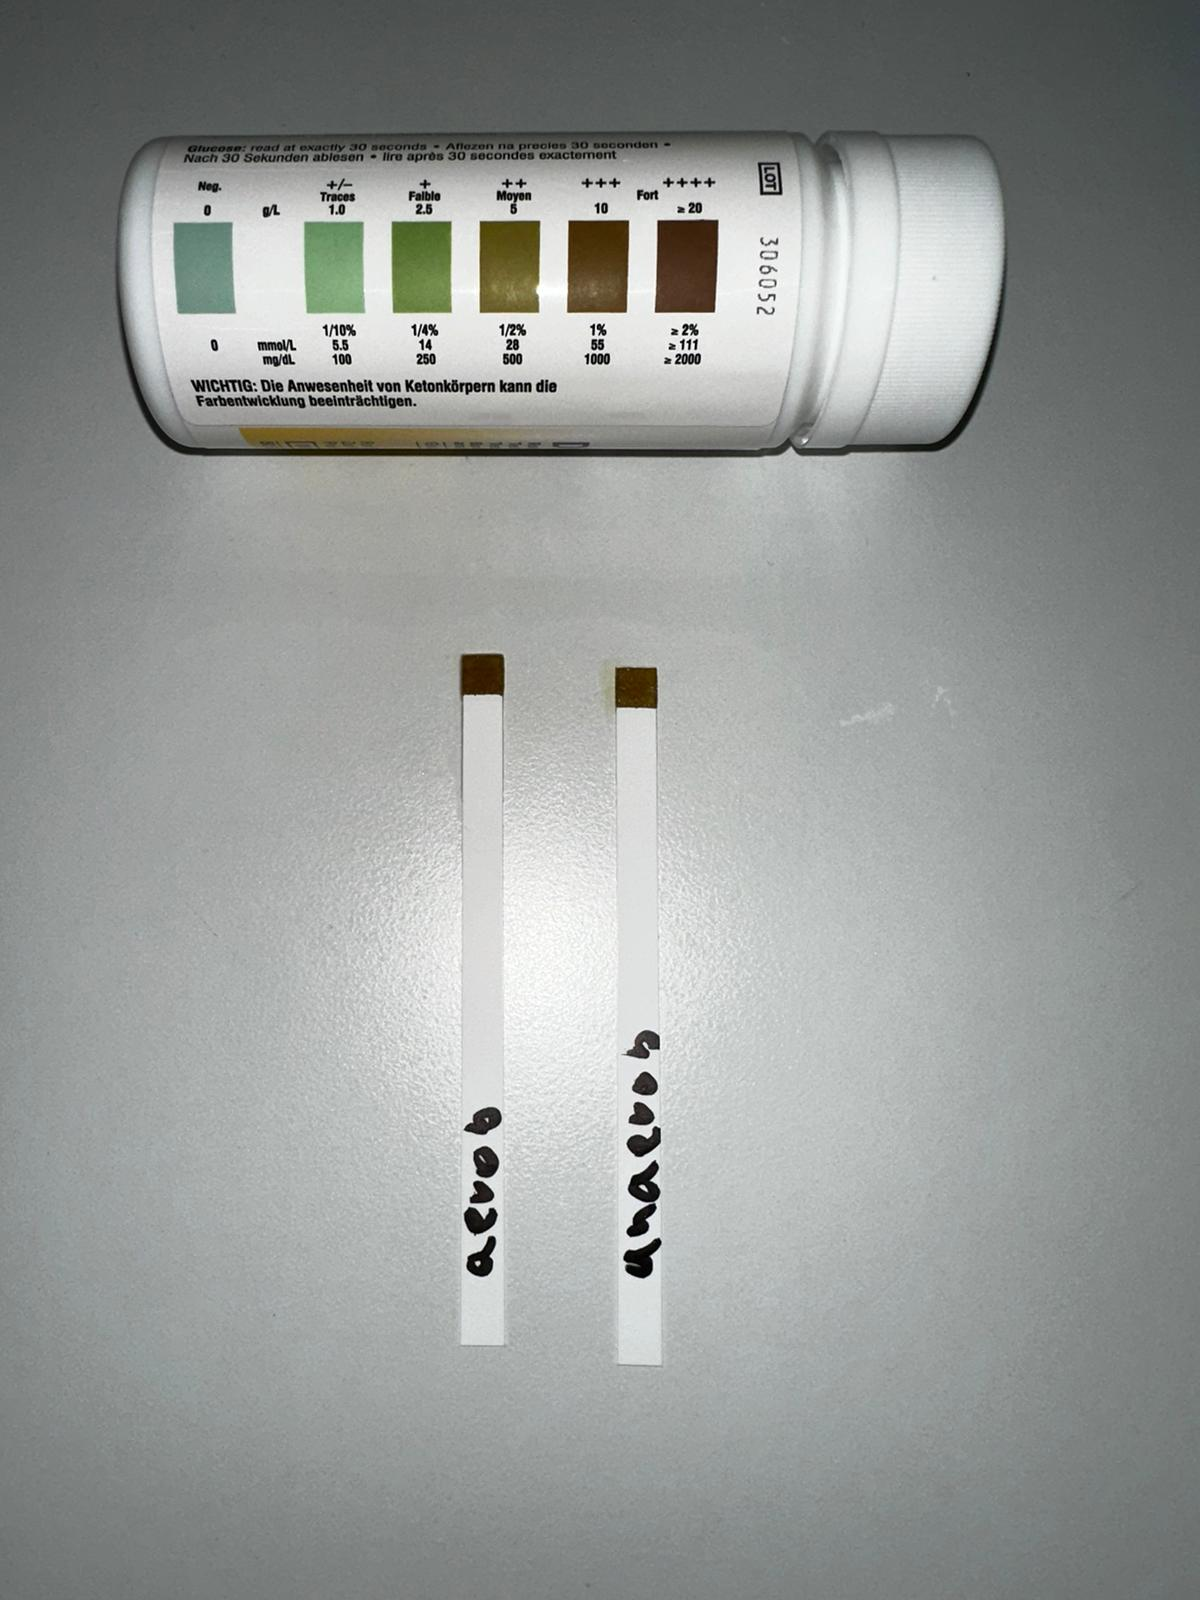
\includegraphics[width=\textwidth]{PHOTO-2024-07-04-23-51-30.jpg}
			\caption{10 Minuten}
			\label{fig:10min}
		\end{subfigure}
		\hfill
		\begin{subfigure}[b]{0.4\textwidth}
			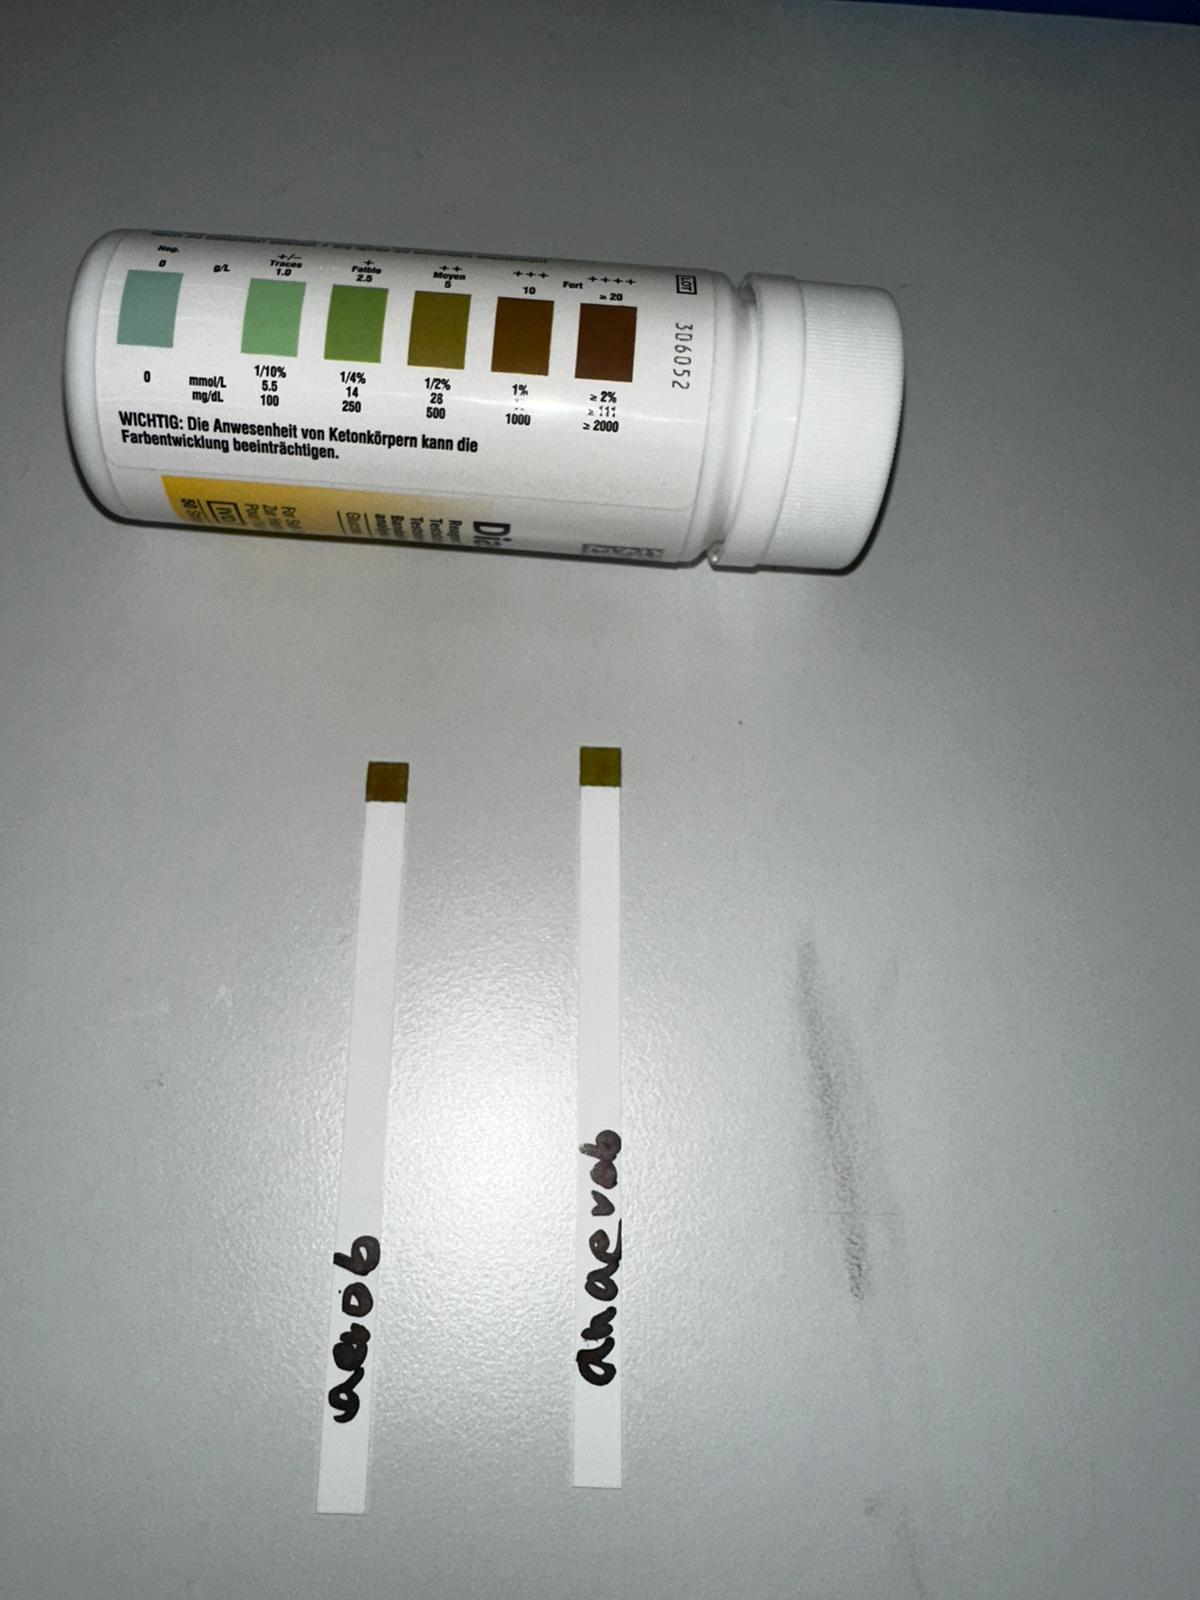
\includegraphics[width=\textwidth]{PHOTO-2024-07-04-23-51-29 2.jpg}
			\caption{15 Minuten}
			\label{fig:15 min}
		\end{subfigure}
		\begin{subfigure}[b]{0.4\textwidth}
			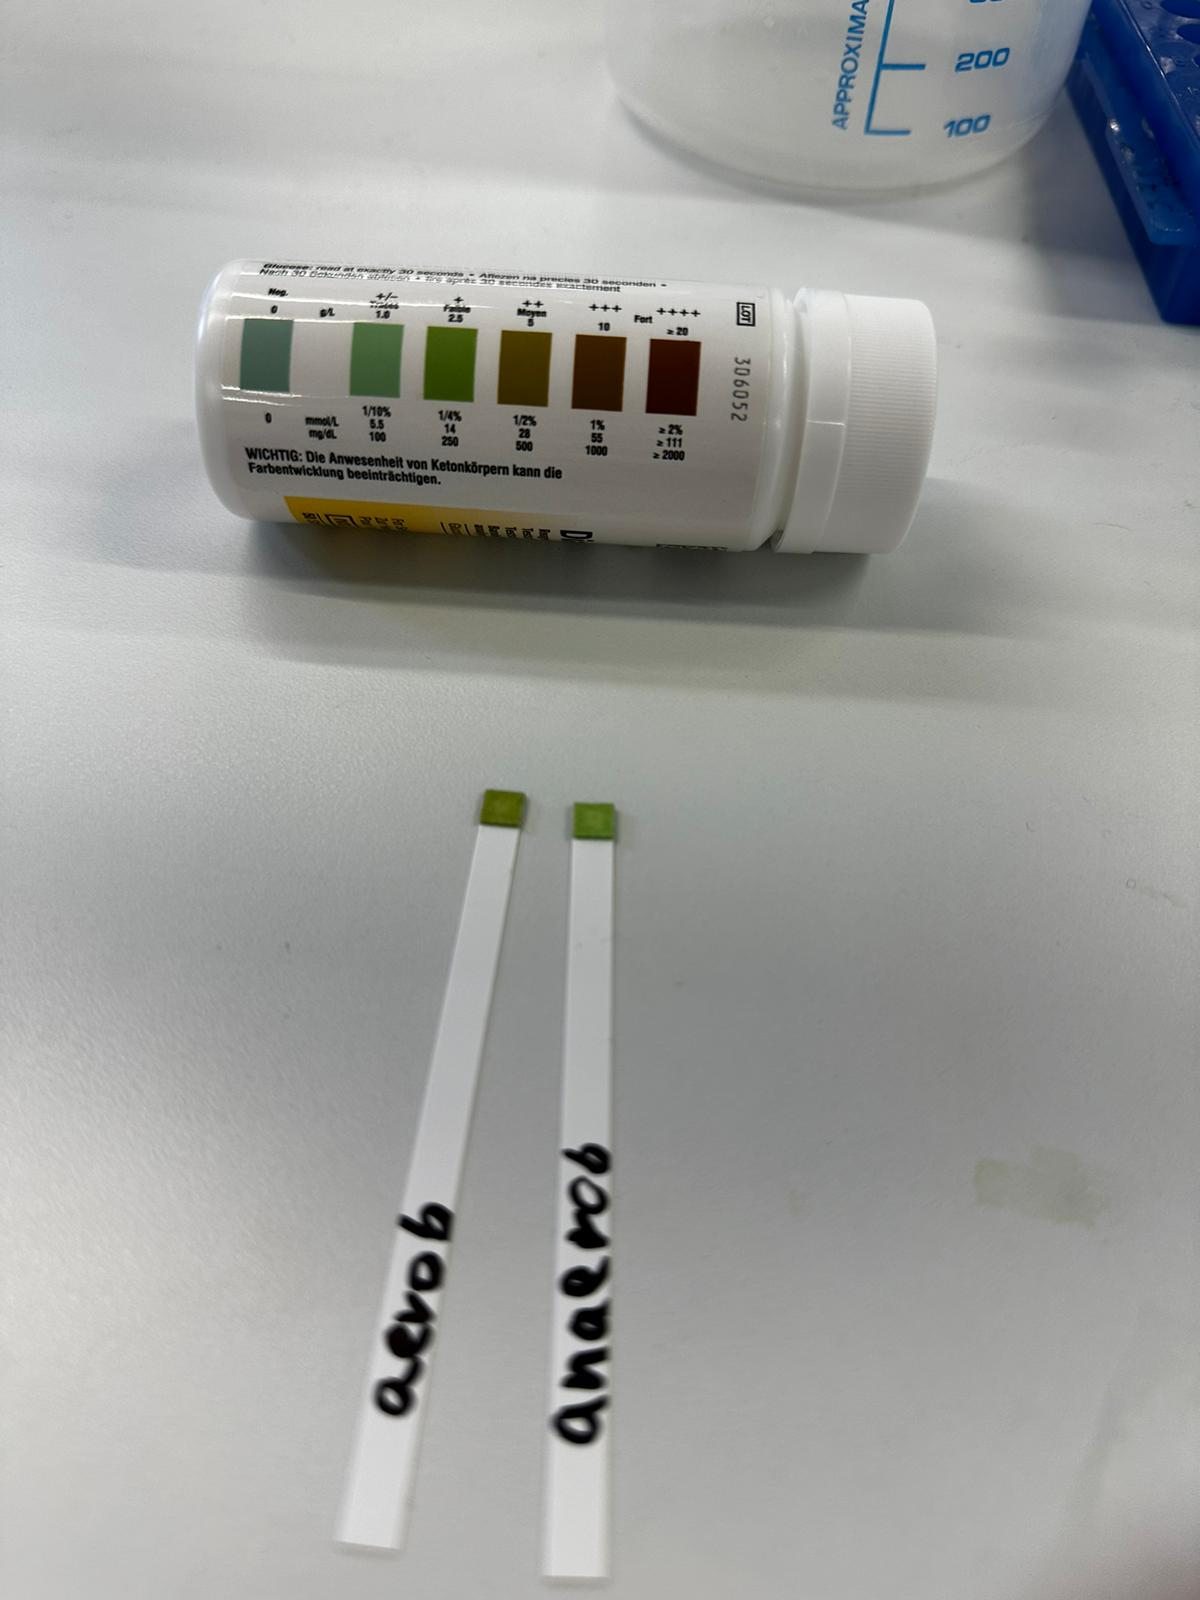
\includegraphics[width=\textwidth]{PHOTO-2024-07-04-23-51-28 2.jpg}
			\caption{20 Minuten}
			\label{fig:20 min}
		\end{subfigure}
		\hfill
		\begin{subfigure}[b]{0.4\textwidth}
			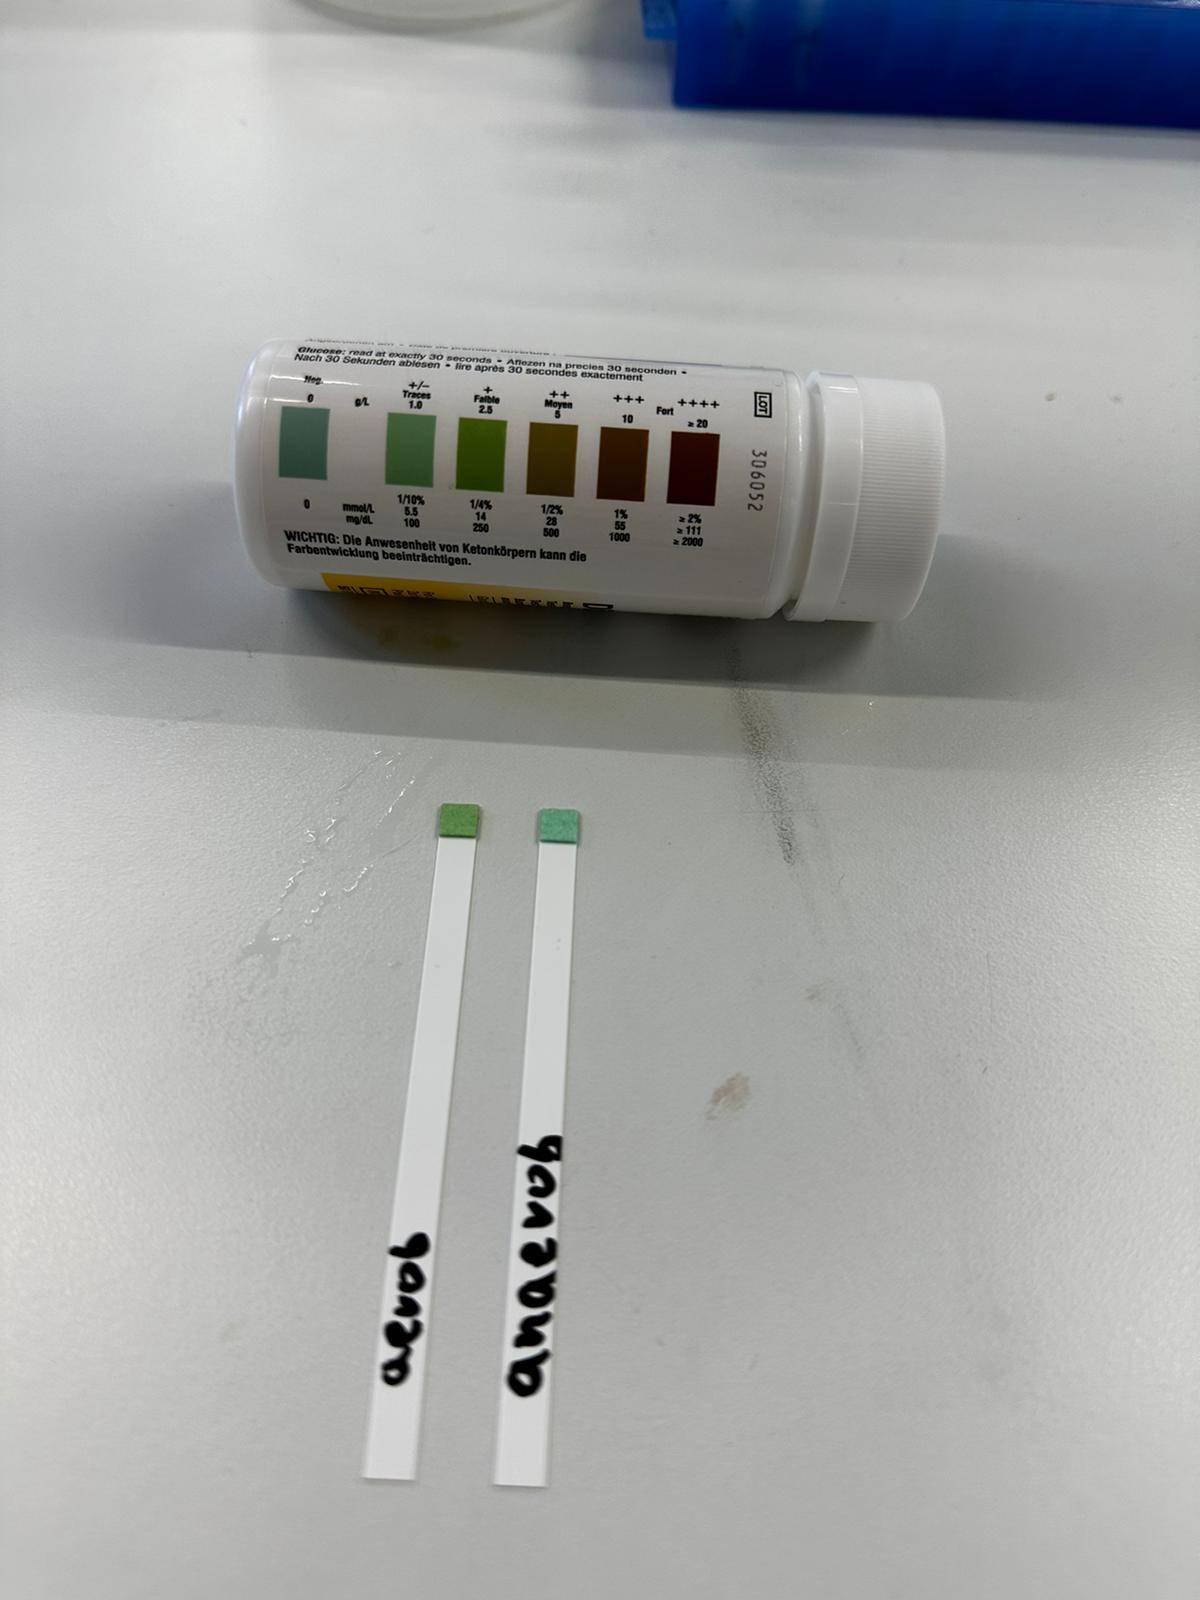
\includegraphics[width=\textwidth]{PHOTO-2024-07-04-23-51-29.jpg}
			\caption{25 Minuten}
			\label{fig:25 min}
		\end{subfigure}
		\caption{Teststreifen nach 10, 15, 20, 25 Minuten in den Backhefe-Lösung bei aerobe und anaerobe Bedingungen.}
		\label{fig: Glucoseverbrauch}
	\end{figure}
	
	\subsubsection{Sauerstoffkonzentrationsmessung}		
	\begin{table}[H]
		\centering
		\caption{Sauerstoffkonzentration von 0.52g Backhefe in einer anaeroben Bedingung.}
		\label{tab:O2 Backhefe ohne KCN}
		\begin{tabular}{cc}
			\toprule
			t in min& ß($O_2$) in mg/L\\
			\midrule
			1.30 & 5.90\\
			2.00 & 5.0\\
			2.30 & 5.34\\
			3.00 & 5.07\\
			3.30 & 4.84 \\
			4.00 & 4.54 \\
			4.30 & 4.30 \\
			5.00 & 4.03 \\
			6.00 & 3.50 \\
			6.30 & 3.23\\
			7.00 & 2.95\\
			7.30 & 2.66\\
			8.00 & 2.38\\
			8.30 & 2.10 \\
			9.00 & 1.84\\
			9.30 & 1.56 \\
			10.00 & 1.29\\
			10.30 & 1.01\\
			11.00 & 0.74\\
			11.30 & 0.47\\
			12.00 & 0.21\\
			12.30 & 0.05\\
			13.00 & 0.00\\			
			\bottomrule
		\end{tabular}
	\end{table}	
	
	\begin{table}[H]
		\centering
		\caption{Sauerstoffkonzentration von 0.52g Backhefe in einer anaeroben Bedingung und Zugabe von 2.4mL 10mM Kaliumcyanid.}
		\label{tab:O2 Backhefe mit KCN}
		\begin{tabular}{cc}
			\toprule
			t in min& ß($O_2$) in mg/L\\
			\midrule
			0.30 & 5.85\\
			1.00 & 5.56\\
			1.30 & 5.49\\
			2.00 & 5.49\\
			2.30 & 5.19 \\
			3.00 & 5.12 \\
			3.30 & 5.08 \\
			4.00 & 5.03\\
			4.30 & 4.97\\
			5.00 & 4.94 \\
			5.30 & 4.89\\
			6.00 & 4.84\\
			6.30 & 4.81\\
			7.00 & 4.77 \\
			7.30 & 4.72\\
			\bottomrule
		\end{tabular}
	\end{table}	
	
	\begin{table}[H]
		\centering
		\caption{Sauerstoffkonzentration von 5.25g BY2-Zellen in einer anaeroben Bedingung.}
		\label{tab:O2 BY2 ohne KCN}
		\begin{tabular}{cc}
			\toprule
			t in min& ß($O_2$) in mg/L\\
			\midrule
			0.30 & 8.09\\
			1.00 & 8.03\\
			1.30 & 7.96\\
			2.00 & 7.93\\
			2.30 & 7.87 \\
			3.00 & 7.83 \\
			3.30 & 7.82 \\
			4.00 & 7.73\\
			4.30 & 7.69\\
			5.00 & 7.64 \\
			\bottomrule
		\end{tabular}
	\end{table}	
	
	\begin{table}[H]
		\centering
		\caption{Sauerstoffkonzentration von 5.25g BY2-Zellen in einer anaeroben Bedingung und Zugabe von 2.4mL 10mM Kaliumcyanid.}
		\label{tab:O2 BY2 mit KCN}
		\begin{tabular}{cc}
			\toprule
			t in min& ß($O_2$) in mg/L\\
			\midrule
			0.30 & 7.61\\
			1.00 & 7.56\\
			1.30 & 7.48\\
			2.00 & 7.41\\
			2.30 & 7.36 \\
			3.00 & 7.30 \\
			3.30 & 7.23 \\
			4.00 & 7.16\\
			4.30 & 7.08\\
			5.00 & 7.01 \\
			\bottomrule
		\end{tabular}
	\end{table}	
	\subsubsection{Graphische Darstellung Sauerstoffverbrauch}
	
		\begin{figure}[H]
		\centering
		\begin{subfigure}[b]{0.5\textwidth}
			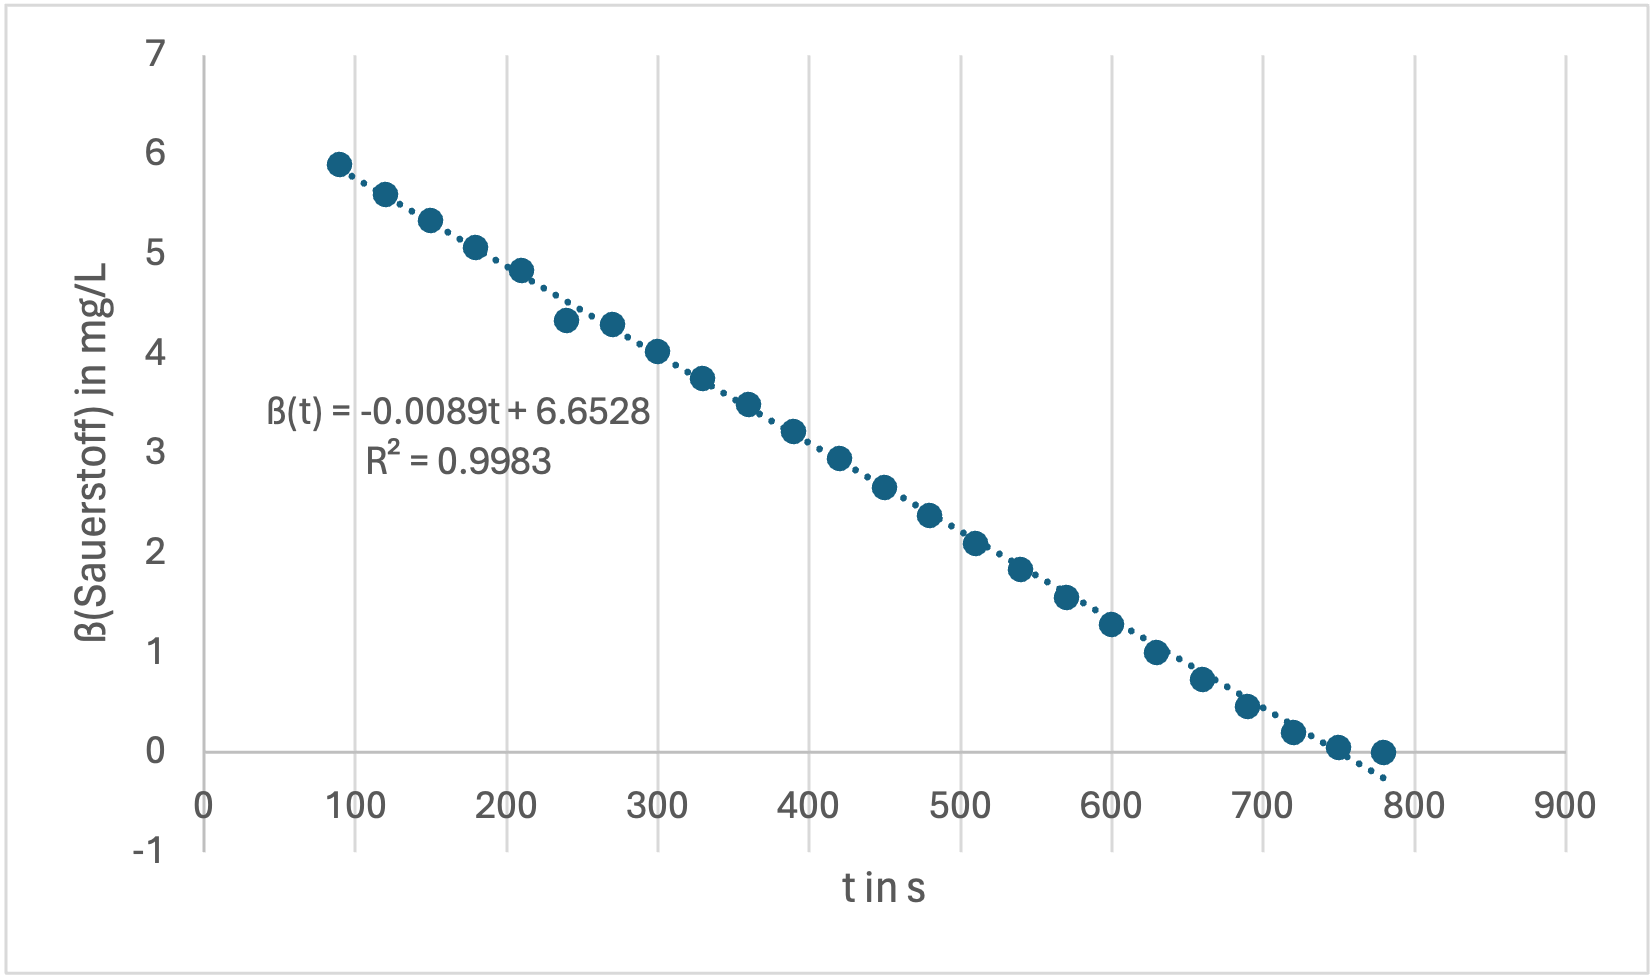
\includegraphics[width=\textwidth]{O2hefeohneKCN.png}
			\caption{Backhefe ohne KCN}
			\label{fig:hefeohneKCN}
		\end{subfigure}
		\hfill
		\begin{subfigure}[b]{0.5\textwidth}
			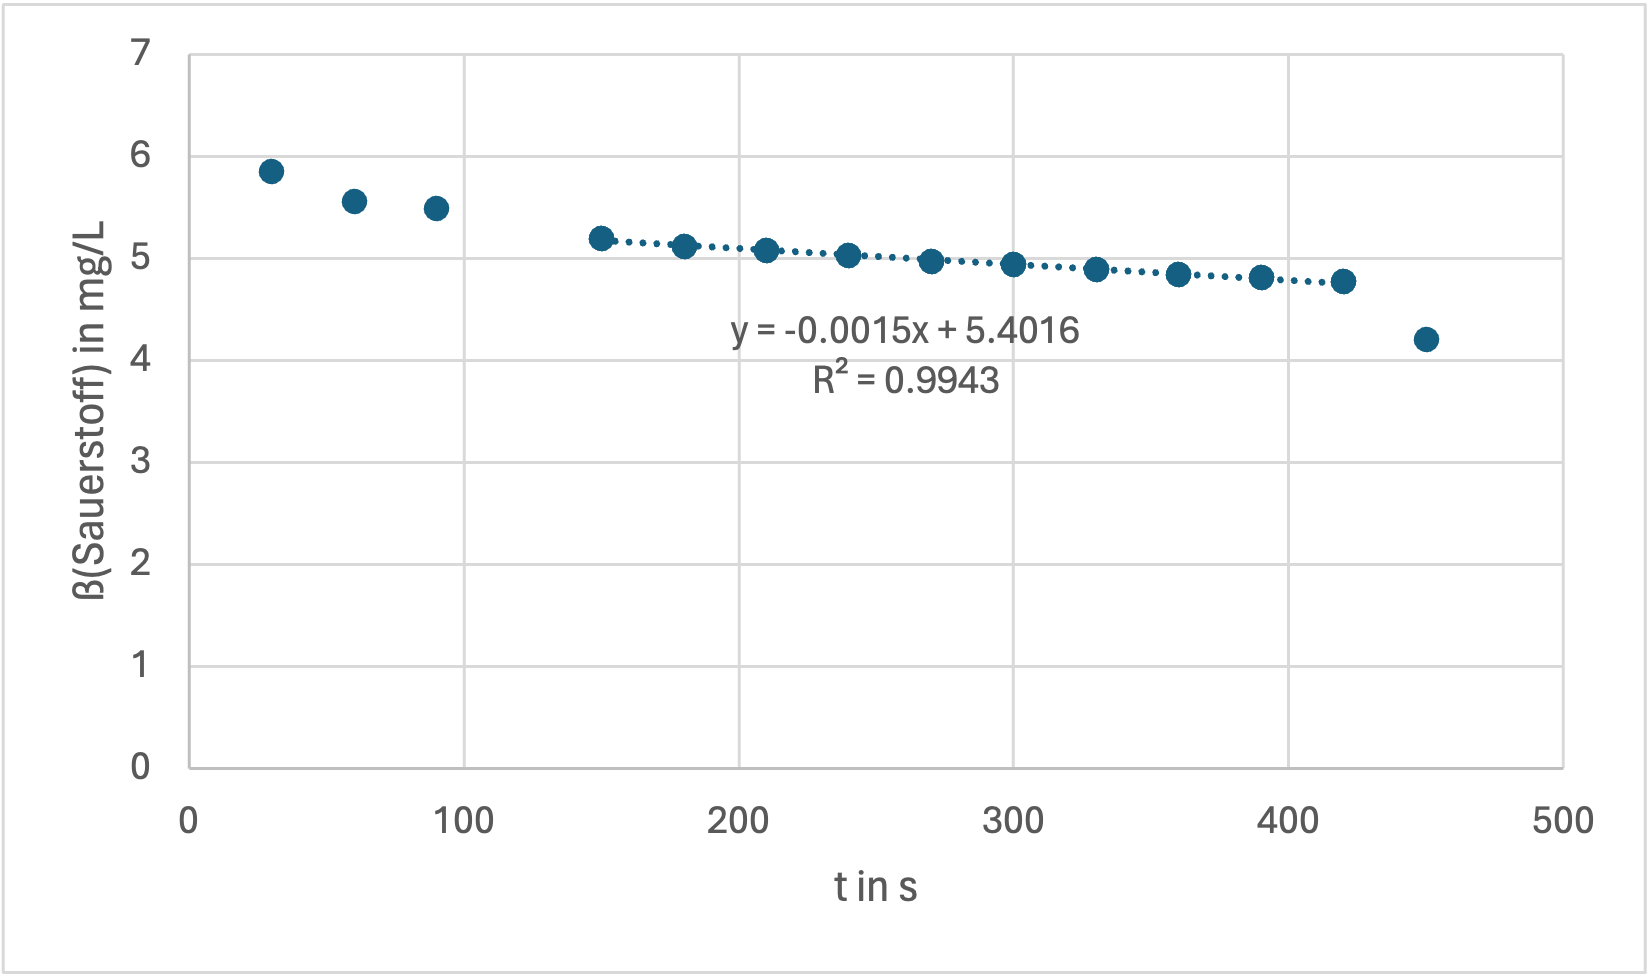
\includegraphics[width=\textwidth]{O2hefemitKCN.png}
			\caption{Backhefe mit KCN}
			\label{fig:hefemitKCN}
		\end{subfigure}
		\begin{subfigure}[b]{0.5\textwidth}
			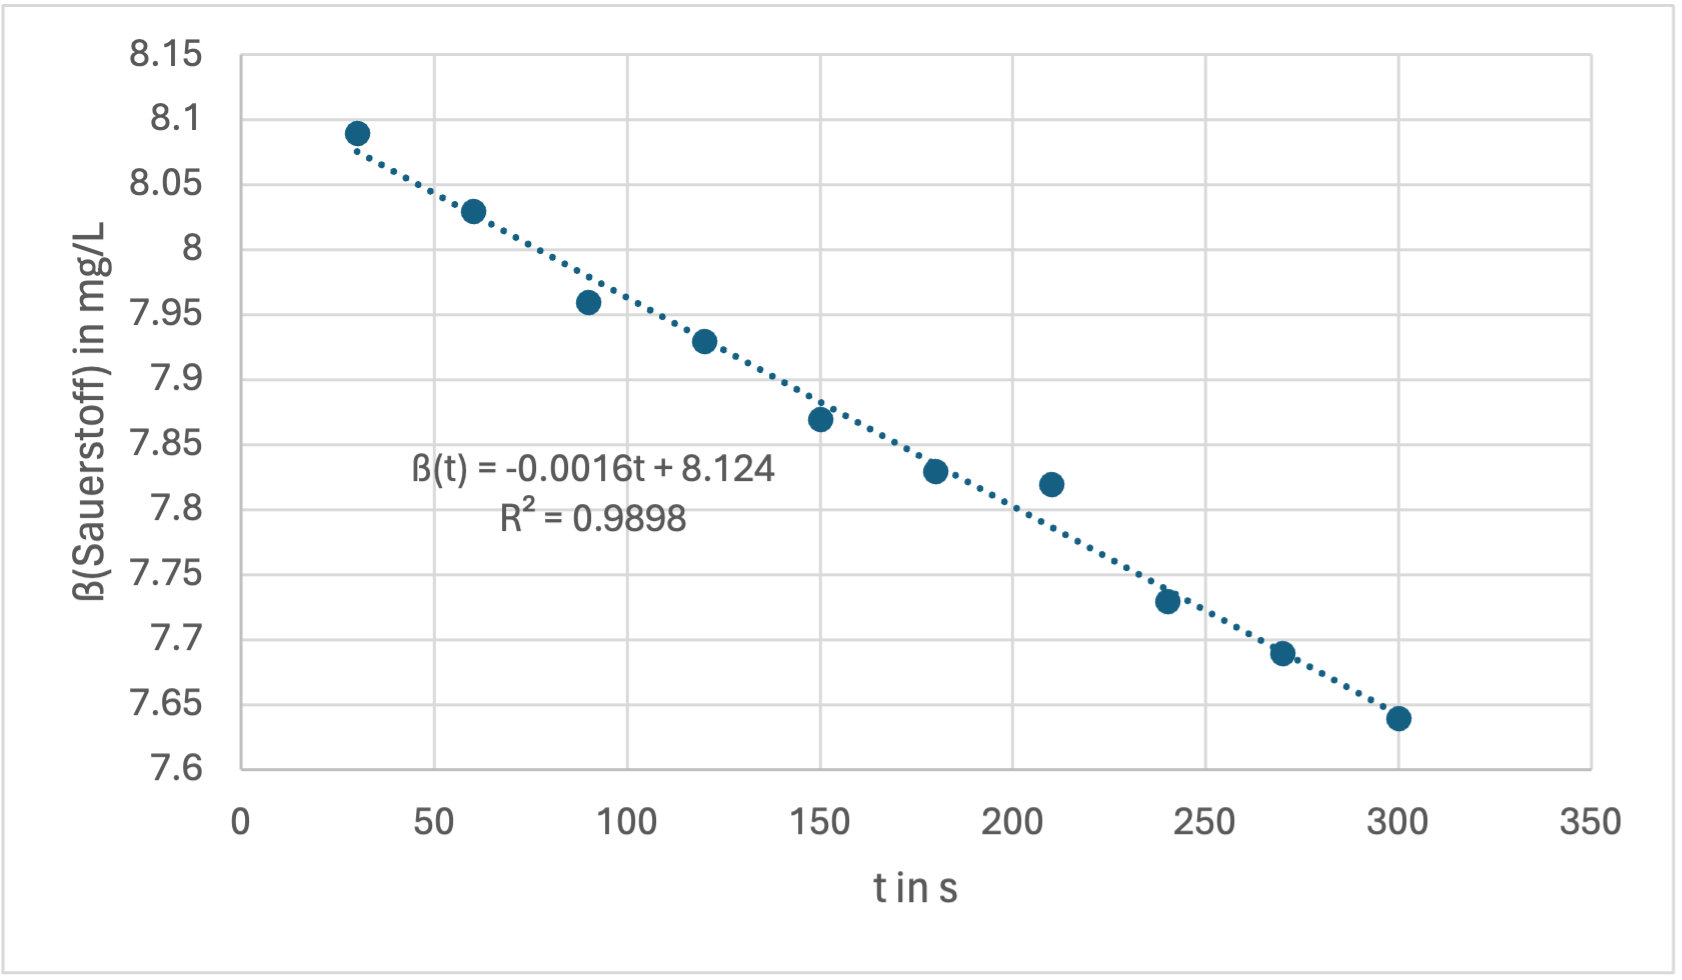
\includegraphics[width=\textwidth]{O2BY2ohneKCN.png}
			\caption{BY2-Zellen ohne KCN}
			\label{fig:BY2ohneKCN}
		\end{subfigure}
		\hfill
		\begin{subfigure}[b]{0.5\textwidth}
			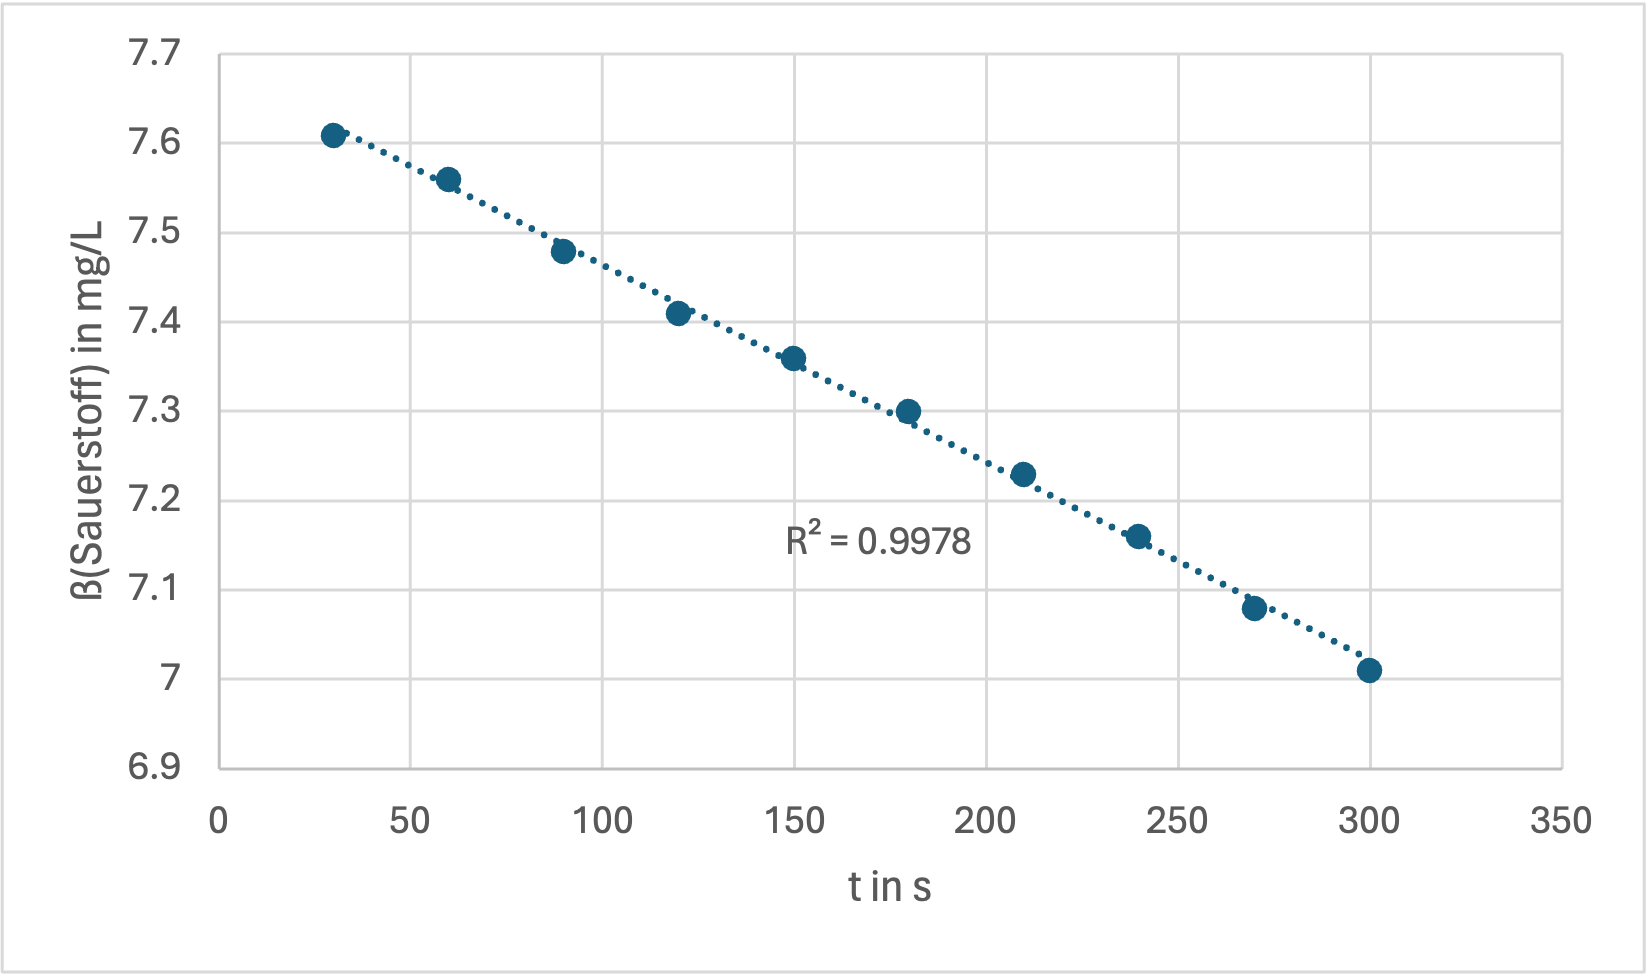
\includegraphics[width=\textwidth]{O2BY2mitKCN.png}
			\caption{BY2-Zellen mit KCN}
			\label{fig:BY2mitKCN}
		\end{subfigure}
		\caption{Sauerstoffkonzentration im Medium von Backhefe bzw BY2-Pflanzenzellen in Abhängigkeit der Zein in Sekunden. Sauerstoffkonzentration wurde in anaerobe Bedingung bestimmt und einmal mit und ohne Zugabe von 2.4mL KCN.}
		\label{fig: Sauerstoffverbrauch}
	\end{figure}
	
	
\end{document}